\clearpage
\subsection{Process View}
\label{subsec:view-process}

\copied{Process view : The process view deals with the dynamic aspects of the system, explains the system processes and how they communicate, and focuses on the runtime behavior of the system. The process view addresses concurrency, distribution, integrators, performance, and scalability, etc. UML Diagrams to represent process view include the Activity diagram.}
{from wikipedia}
This view mainly discuss about runtime, concurrency, communication, and synchronization of the process running in the system. \\

The program flow and business logic of the system are captured in this section with the aid of activity and sequence diagrams.

\subsubsection*{Flood monitoring}
\label{subsubsec:proc-floodmonitor}

The activity diagram in Figure~\ref{fig:activity-monitoring} shows the flow of the flood monitoring process. The boxes represent different parts of the system. The black dots with and without a thin black circle around them represent the begin and end of a process respectively.

Figure~\ref{fig:activity-controlpanel} shows another activity diagram. This one displays the processes relating to the control panel.


\begin{figure}[H]
	\centering
	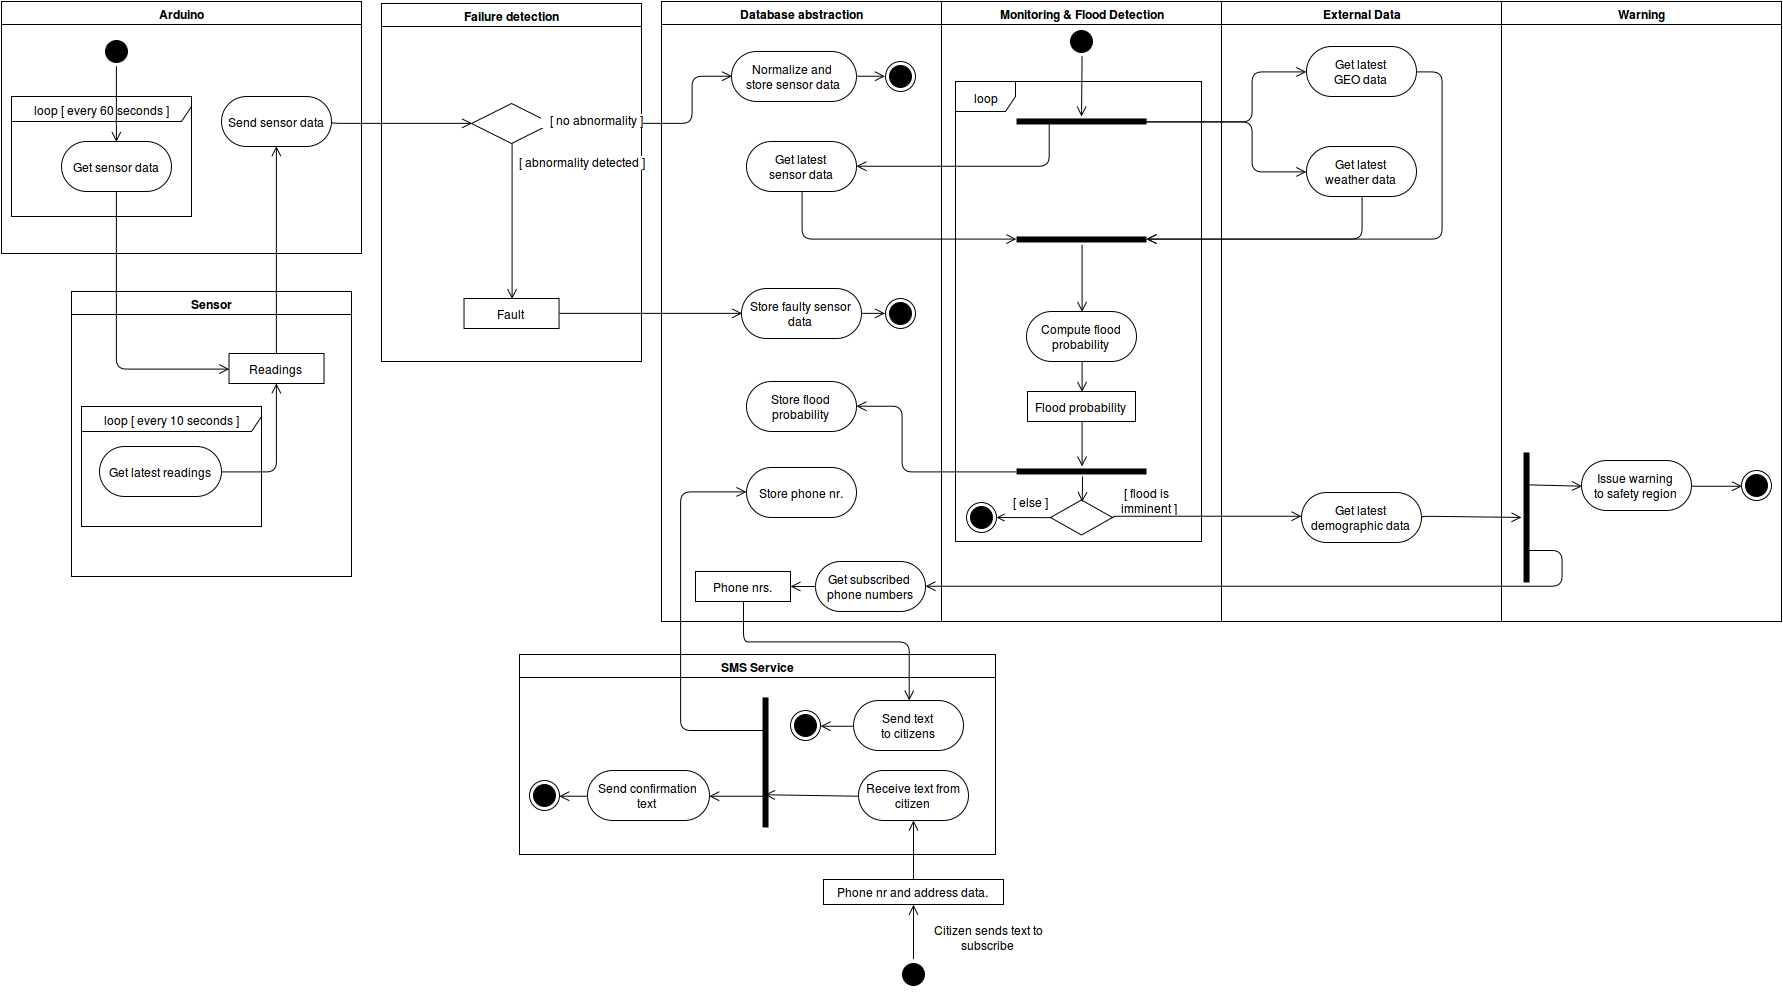
\includegraphics[keepaspectratio=true,width=1.0\textwidth]{{\viewimages/activity_monitoring}.png}
	\caption{An activity diagram of the flood monitoring process}
	\label{fig:activity-monitoring}
\end{figure}

\begin{figure}[H]
	\centering
	\includegraphics[keepaspectratio=true,width=0.55\textwidth]{{\viewimages/control-panel}.png}
	\caption{An activity diagram of the control panel}
	\label{fig:activity-controlpanel}
\end{figure}